\section{\AP{}Intermezzo: Tagged Tree Decompositions}
\label{sec:treedec}

In this section we introduce some technical tools necessary for the proof of
the "Key Lemma". Remember that its statement deals with
\[
	\MUAHomBounded{\gamma}{\Tw}{\leq m} \defeq 
    \{ 
        \alpha \in \Tw
        \mid
        \exists \rho \in \Refin[\leq m](\gamma),\, \exists \fun\colon \rho \surj \alpha
    \},
\]
and consequently its proof needs to manipulate "homomorphisms"
from "refinements" onto "C2RPQs" of "tree-width" $\leq k$.
The proof will ``massage'' the "homomorphism" $f$ and queries $\alpha,\rho$ in order to reduce the size of $m$, while preserving (a) the existence of a "homomorphism" between the two queries,
(b) the "tree-width" of the right-hand side, (c) the fact that the left-hand side is a "refinement",
and (d) some semantic properties of the queries. Our construction will be guided by
the "tree decomposition" of $\alpha$, and more importantly by how $\rho$ is mapped onto such decomposition.

\begin{figure}[tbp]
	\centering
	\subfloat[A query $\gamma$ of "tree-width" 3.]{%
		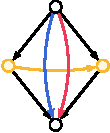
\includegraphics[width=.25\linewidth]{trio-query.pdf}
	}
	\hfill
	\subfloat[A "refinement" $\rho$ of $\gamma$.]{%
		\AP\label{fig:trio-refinement}
		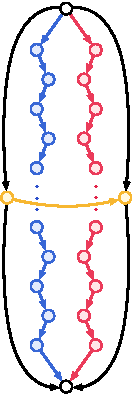
\includegraphics[width=.35\linewidth]{trio-refinement.pdf}
	}
	\hfill
	\subfloat[A homomorphic image $\alpha$ of $\rho$ of "tree-width" 2. See \Cref{fig:trio-tree-dec} for a "tree decomposition" of $\alpha$ (ignoring the dashed blue lines).]{%
		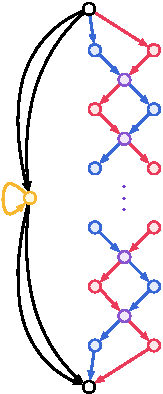
\includegraphics[width=.35\linewidth]{trio-approximation.pdf}
	}
	\caption{
		\AP\label{fig:trio}
		An example of a "homomorphism" $f\colon \rho \surj \alpha$.
		The "strong onto homomorphism" $f$ is implicitly defined: it sends the two yellow
		vertices of $\rho$ on the unique yellow vertex of $\alpha$, and identifies some
		blue and red vertices of $\rho$---thus creating purple vertices in $\alpha$.
	}
\end{figure}

\begin{definition}
    \AP Let $\fun\colon \rho \homto \alpha$ be a "homomorphism" between two "C2RPQs".
    A ""tagged tree decomposition""
    of $\fun$ is a triple $(T, \bagmap, \intro*\tagmap)$ where
    $\tup{\?T, \bagmap}$ is a "tree decomposition" of $\alpha$,
    and $\tagmap$ is a mapping $\tagmap\colon \atoms{\rho} \to \vertex{\?T}$, called \AP""tagging"",
    such that for each "atom" $e = x \atom{\lambda} y \in \atoms{\rho}$, we have that $\bagmap(\tagmap(e))$ "contains@@tw" both $\fun(x)$ and
    $\fun(y)$.
\end{definition}

\begin{figure}[tbp]
	\centering
	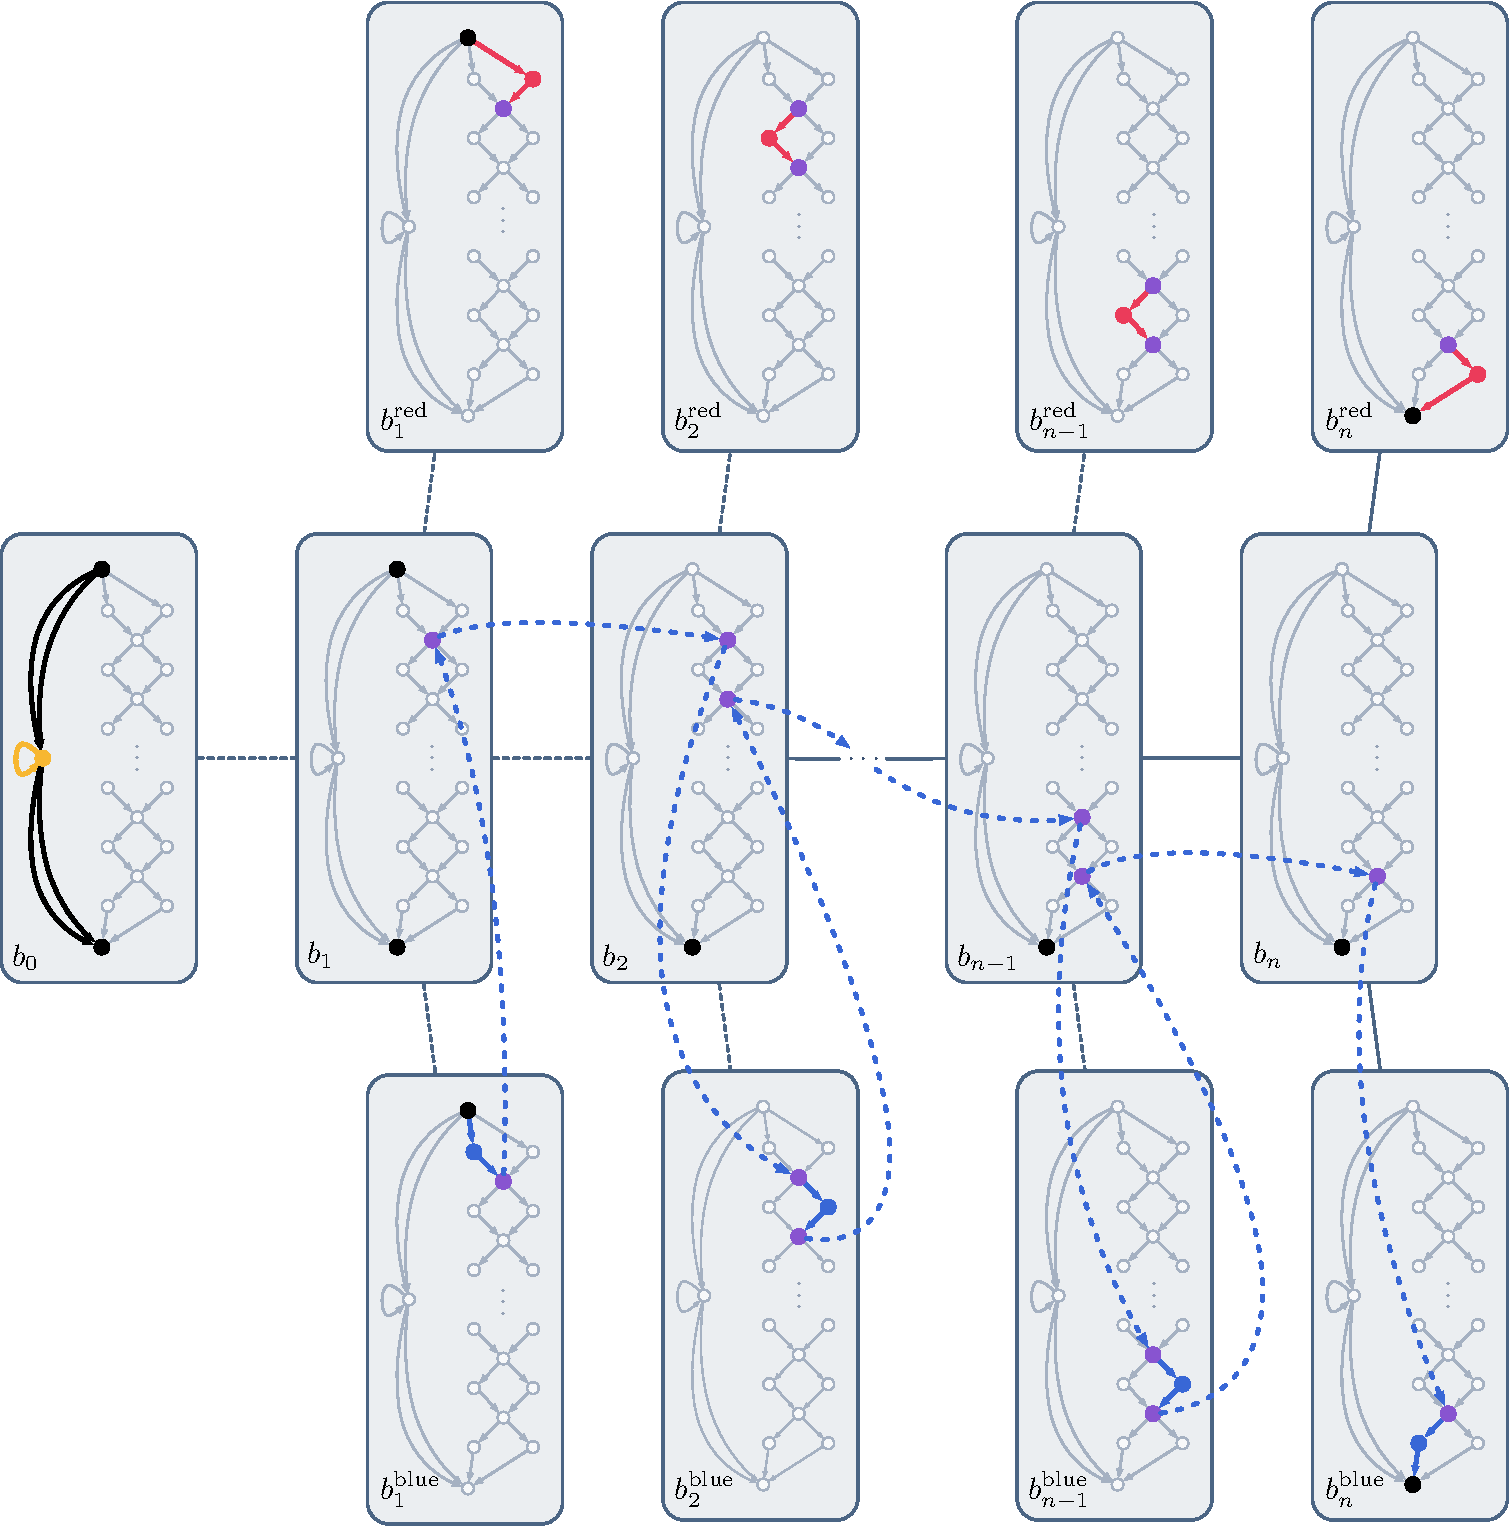
\includegraphics[width=\linewidth]{trio-tree-dec.pdf}
	\caption{
		\AP\label{fig:trio-tree-dec}
		A "fine tagged tree decomposition" of $\alpha$ (see \Cref{fig:trio}) of "width" 2.
		(Recall that some bags are omitted for the sake of readability. These bags
		are there to make the decomposition "fine".)
	}
\end{figure}

In other words, $\tagmap$ gives,
for each "atom" of $\rho$, a witnessing "bag" that "contains@@tw" it, in the sense that
it contains the image by $\fun$ of the atom's source and target.
By definition, given a "tree decomposition" $\tup{\?T, \bagmap}$ of $\alpha$ and a "homomorphism"
$\fun\colon \rho \surj \alpha$, there is always one way (usually many) of extending $\tup{\?T, \bagmap}$
into a "tagged tree decomposition" of $\fun$.

We provide an example of "homomorphism" $\fun\colon \rho \surj \alpha$ in \Cref{fig:trio}. Note 
that in this example, $\rho$ is defined as the "refinement" of a query, and $\fun$ is "strong 
onto"---for now this is innocuous, but we will always work under these
assumptions in \Cref{sec:proof-key-lemma}. In \Cref{fig:trio-tree-dec}, we give a "tagged tree 
decomposition" of this "homomorphism". Each "bag" is given a name, written in the bottom left 
corner. The "tagging" is represented as follows: if an "atom" is "tagged" in a "bag", then it
is drawn as a solid bold arrow in this "bag". Note that by definition, a given "atom" is "tagged" in
exactly one "bag". For now, blue dashed arrow between bags can be ignored---they will illustrate \Cref{def:path-induced}.

\begin{fact}
    \AP\label{fact:restriction_tagged_treedec}
    Let $(T, \bagmap, \tagmap)$ be a "tagged tree decomposition" of some "strong onto homomorphism"
    $\fun\colon \rho \surj \alpha$.
    Let $T'$ be the smallest connected subset of $T$ containing the image of $\tagmap$.
    Then $(T', \bagmap\vert_{T'}, \tagmap)$ is still a "tagged tree decomposition" of $\fun$,
    whose "width" is at most the "width" of $(T, \bagmap, \tagmap)$.
\end{fact}

% \begin{figure}[htb]
%     \centering%
%     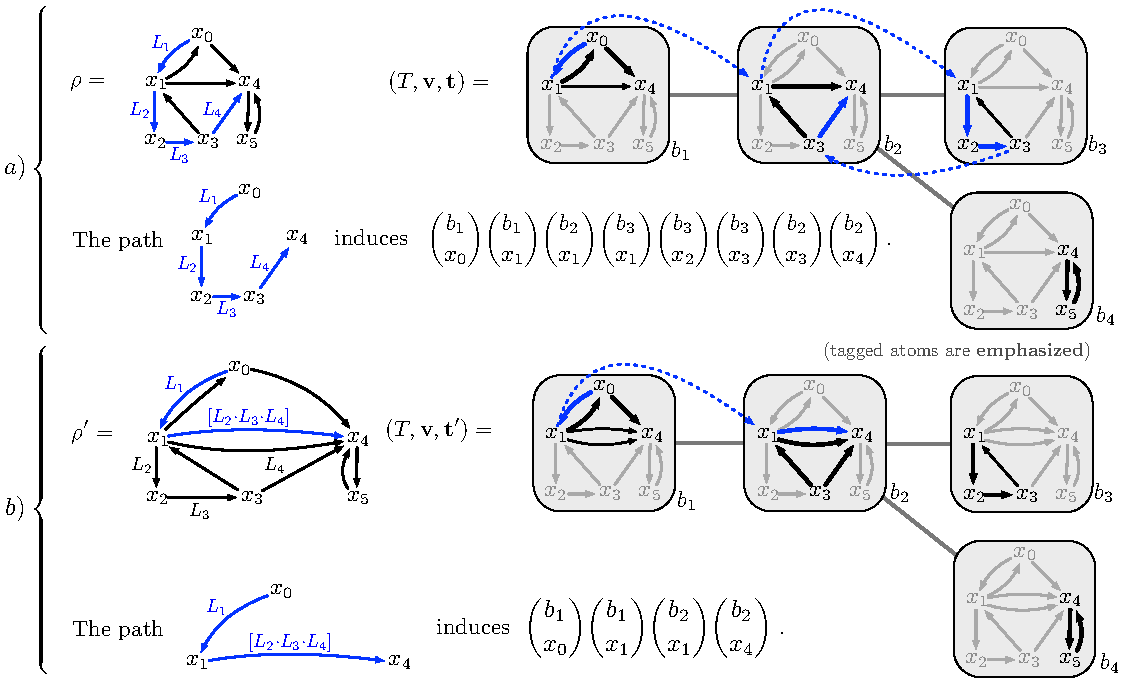
\includegraphics[width=\linewidth]{path-induced.pdf}
%     \caption{%
%         \AP\label{fig:path-induced}%
%         $a)$ Non-"acyclic path" "induced" by some path in $\rho$ (left-hand side), in a "tagged tree decomposition" (right-hand side) of $\fun\colon \rho \homto \alpha$ in the case where $\alpha = \rho$ and $\fun$ is the identity "homomorphism" $\textrm{id}_\rho\colon \rho \homto \rho$.\\
%         $b)$ Suppose that the path in $\rho$ is the image of an "atom refinement" of $\gamma$. Then the cycle in the induced path can be avoided by adding an "atom" $x_1 \atom{\contract{L_{2} \cdot L_3 \cdot L_4}} x_4$ to $\rho$, obtaining the path of $\rho'$,
%         whose "induced path" is "acyclic@@path".
% 		\remi{Todo: remove fig?}
%     }
% \end{figure} 

In the following paragraphs, we extend the notion of "tagging" to paths.
We illustrate this notion in \Cref{fig:trio-tree-dec}, where we describe
the path induced by
the blue path of \Cref{fig:trio-refinement}---which starts at the top-most vertex,
follows the blue atoms, and reaches the bottom-most vertex.
\AP Informally, in the context of a "tagged tree decomposition" $(T, \bagmap, \tagmap)$ of  $\fun\colon \rho \homto \alpha$, given a path $\pi$ of $\rho$, say $x_0 \atom{\lambda_1} x_1 \atom{\lambda_2} \cdots \atom{\lambda_n} x_n$, the "path induced" by $\pi$, denoted by $\tagmappath{\pi}$, is informally defined as the following ``path'' in
$T\times \alpha$, seen as a sequence of pairs of "bags" and variables
from $V(T) \times \vars(\alpha)$:
\begin{itemize}
    \item it starts with the "bag" $\tagmap(x_0 \atom{\lambda_1} x_1)$ of $T$ and the variable $\fun(x_0)$ of $\alpha$; in \Cref{fig:trio-tree-dec}, this corresponds to bag $b^{\text{blue}}_1$;
	\item it then goes to $\langle \tagmap(x_0 \atom{\lambda_1} x_1), \fun(x_1) \rangle$;
    \item it then follows the shortest path in $T$ (unique, since it is a tree) that goes to the "bag" $\tagmap(x_1 \atom{\lambda_2} x_2)$, while staying in $\fun(x_1)$ in $\alpha$---in \Cref{fig:trio-tree-dec}, this bag is the same as before, namely $b^{\text{blue}}_1$, so we do nothing;
    \item then, it goes to $\langle \tagmap(x_1 \atom{\lambda_2} x_2),\fun(x_2) \rangle$ in a single step;
    \item it then follows the shortest path in $T$ (unique, since it is a tree) that goes to the "bag" $\tagmap(x_2 \atom{\lambda_\lambda} x_3)$, while staying in $\fun(x_2)$ in $\alpha$---in our running example, we go from $b^{\text{blue}}_i$
	to $b_i$, and then to $b_{i+1}$ before reaching $b^{\text{blue}}_{i+1}$;
    \item it continues in the same way for all other atoms of the path, ending up with the  "bag" $\tagmap(x_{n-1} \atom{\lambda_n} x_n)$ and the variable $\fun(x_{n})$ of $\alpha$.
\end{itemize}
By construction, note that the constructed sequence $(b_i, z_i)_{i}$,
also denoted by $({b_i \choose z_i})_{i}$, is
such that $z_i \in \bagmap(b_i)$. Moreover, the values taken
by the sequence $(z_i)_{i}$ are $(f(x_j))_{0 \leq j \leq n}$, in the same order
but potentially with repetitions.
Graphically, this sequence corresponds to a path in the "tagged tree decomposition", where one can
not only move along the "bags", but also along the variables they contain.
In our example, the "path induced" by the blue path of \Cref{fig:trio-refinement}
corresponds in \Cref{fig:trio-tree-dec} to the blue path consisting of both solid and dashed edges.
Moreover, note that a single atom $x_0 \atom{\lambda} x_1$ of $\rho$ "induces the path":
\begin{equation}
	\AP\label{eq:path-induced-atom}
	\Bigl\langle
	{\textstyle
		{ \tagmap(x_0 \atom{\lambda} x_1) \choose x_0 },\;
		{ \tagmap(x_0 \atom{\lambda} x_1) \choose x_1 }
	}
	\Bigr\rangle.
	% \tag{\adfast9}
\end{equation}

\begin{definition}[Path induced in a tagged tree decomposition---formal definition]
	\AP\label{def:path-induced}
	Given a "homomorphism" $f\colon \rho \homto \alpha$ and a "tagged tree decomposition"
	$(T, \bagmap, \tagmap)$ of $f$,
    the \AP""link"" from an "atom" $A = x \atom{\lambda} y$ to an "atom" $B= y \atom{\lambda'} z$ of $\rho$ is the unique (possibly empty) sequence
    $
    % \[	
            \textstyle{
                % {\tagmap(A) \choose \fun(y)},\,
                {b_{1} \choose \fun(y)}, \hdots,
                {b_{n} \choose \fun(y)},
                % {\tagmap(B) \choose \fun(y)}
            }
    % \]
    $
    where $\tagmap(A), b_{1}, \dotsc, b_n, \tagmap(B)$ is the unique simple path from $\tagmap(A)$ to $\tagmap(B)$ in $T$.

    \AP The \intro{path induced} by a path
	$
		\pi = 
		x_0 \atom{\lambda_1} x_1 \atom{\lambda_2} \cdots \atom{\lambda_n} x_n
	$
	of $\rho$ is the unique sequence
    \[
		\intro*\tagmappath{\pi} \defeq
            \textstyle{
                {b_0 \choose \fun(x_0)} {b_0 \choose \fun(x_1)} \,
                L_1 \,
                {b_1 \choose \fun(x_1)} {b_1 \choose \fun(x_2)} \,
                L_2 
                \dotsb 
				{b_{n-2} \choose \fun(x_{n-2})}
                L_{n-1} \,
                {b_{n-1} \choose \fun(x_{n-1})} {b_{n-1} \choose \fun(x_n)}
            }
    \]
    where $b_i = \tagmap(x_i \atom{\lambda_{i+1}} x_{i+1})$ and $L_i$ is the "link" from $x_{i-1} \atom{\lambda_i} x_i$ to $x_{i} \atom{\lambda_{i+1}} x_{i+1}$, for every $i$.
\end{definition}

\AP Moreover, given a "bag" $b$ of $T$ and a variable $z$ of $\alpha$, we say that
$\tagmappath{\pi}$ ""leaves"" $b$ at $z$ when ${b \choose z}$ belongs to
$\tagmappath{\pi}$, and this is either the last element of the sequence $\tagmappath{\pi}$,
or the next element of the sequence has a "bag" distinct from $b$.

For example, in \Cref{fig:trio-tree-dec},
$\tagmappath{\pi}$ "leaves" $b^{\text{blue}}_1$ at the first purple vertex.
Similarly, it "leaves" $b_1$ and $b_2$ at this same vertex. Moreover,
it also "leaves" $b_2$ at the second purple vertex.

We say that an "induced path" is \AP""cyclic@@path"" if it contains two positions $i, j$
such that $i+2 \leq j$ and $b_i = b_{j}$.
We say that it is \reintro(path){acyclic} otherwise,
meaning that if we visit a "bag" for the first time, we can visit it again at
most once, in which case it must be precisely at the next time step.
For instance, the "path induced" by the blue "atom refinement" in \Cref{fig:trio-tree-dec}
is "cyclic@@path". However, the "path induced" by a single
"atom"---see \eqref{eq:path-induced-atom}--- is always "acyclic@@path".

\begin{fact}
	\AP\label{fact:acyclic-decomposition-leave-forever}
	If an "induced path" $\tagmappath{\pi}$ is "acyclic@@path", for any "bag" $b$,
	there is at most one variable $z$ of $\alpha$ such that $\tagmappath{\pi}$
	"leaves" $b$ at $z$.
\end{fact}

% \AP Note that any ""non-branching path""---"ie"~a path whose non-extremal "bags" have degree 2---in a "nice tree decomposition" with $n$ "bags" must have at least $\lfloor n/2 \rfloor$ "bags" which are not "full"\footnote{This worst-case being reached by alternating between removing and adding a vertex to the bag.}.
\AP Lastly, we define a ""fine tagged tree decomposition"" of $\fun\colon \rho \homto \alpha$
to be a "tagged tree decomposition" of $\fun$ that is also a "fine tree decomposition" of $\alpha$.
We abuse the notation and talk about the "fine tagged tree decomposition" of a "C2RPQ" $\gamma$
to talk about the "fine tagged tree decomposition" of the identity "homomorphism"
$\id\colon \gamma \surj \gamma$.

\AP One of the key properties of "fine tagged tree decompositions" is that in any of its ""non-branching paths""---"ie" paths in $T$ whose non-extremal "bags" have degree exactly 2---, at least half of the "bags" are "non-full", "ie" they
contain at most $k$ variables\footnote{Recall 
that in a decomposition of "width" $k$, "bags" are allowed to contain at most $k+1$ variables.}.
Such "bags" will prove useful in the next section because of the following property.

\begin{figure}
    \centering
    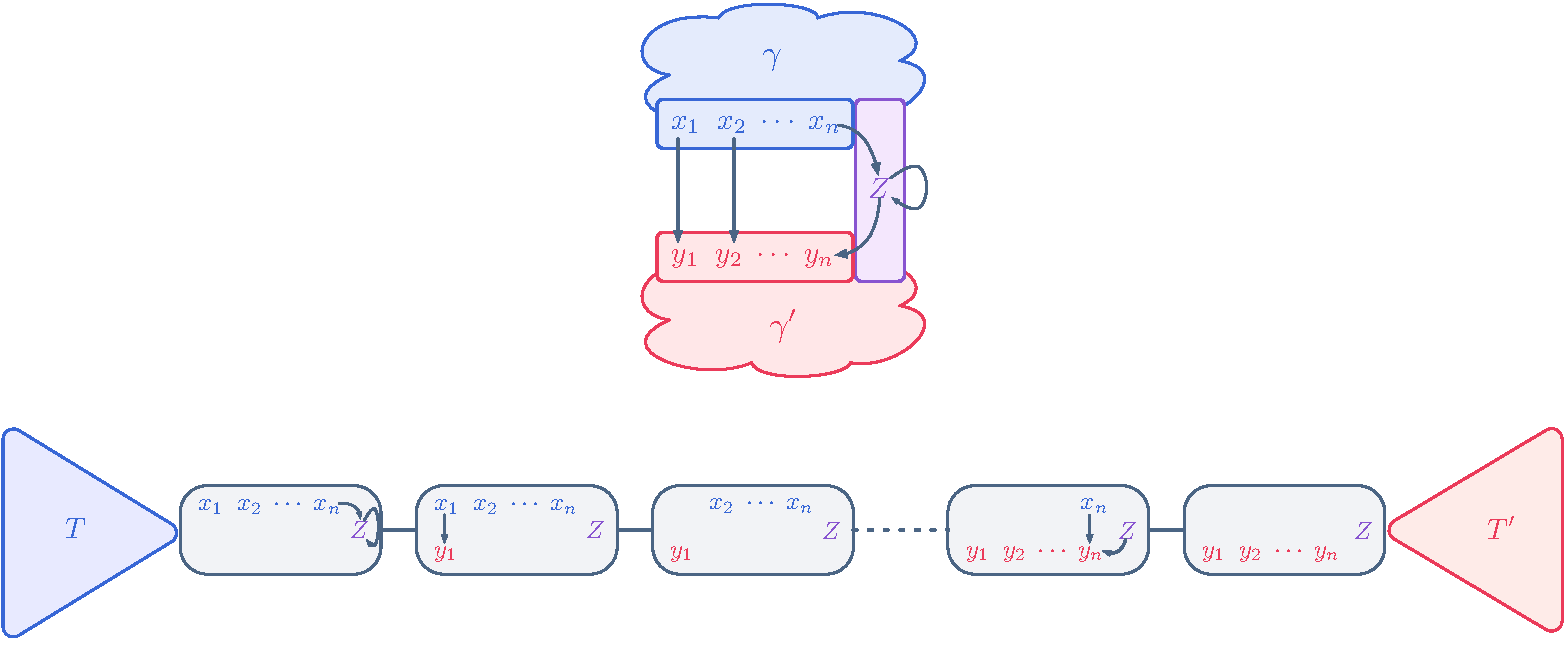
\includegraphics[width=\linewidth]{connecting-tree-decompositions.pdf}
    \caption{%
        \AP\label{fig:connecting-tree-decompositions} The query
        $\gamma \land \gamma' \land \delta$ (top)
        and one of its "fine tagged tree decomposition"
		of "width" at most $k$ (bottom).
    }
\end{figure}

\begin{proposition}
    \AP\label{prop:connecting-tree-decompositions}
    Let $\gamma,\gamma'$ be "C2RPQs",
    and $(T,\bagmap,\tagmap)$---resp.\ $(T',\bagmap',\tagmap')$---be
	a "fine tagged tree decomposition" of width $k$ of $\gamma$---resp.\ of $\gamma'$.
    Let $b, b'$ be leaves of $T$ and $T'$ respectively, such that $b$ and $b'$ are "non-full bags"
	of the same cardinality,
	and let $Z = \bagmap(b) \cap \bagmap'(b')$. In particular, we have
	% Let $Z$ be the set of variables in common between $\bagmap(b)$ and $\bagmap'(b')$, so that we have
    \[
        \bagmap(b) = \{x_1,\hdots,x_n\}\cup Z
        \;\text{ and }\;
        \bagmap'(b') = \{y_1,\hdots,y_n\}\cup Z,
    \]
	from some variables "st" the $x_i$'s are disjoint from the $y_i$'s.
	Assume moreover that $\vars(\gamma) \cap \vars(\gamma') \subseteq Z$.
    Then, for any conjunction $\delta$ of "atoms" the form:
	\begin{itemize}
		\item $x_i \atom{L} y_i$ for some $i \in \lBrack 1, n \rBrack$,
		\item $x_i \atom{L} z$ for some $i \in \lBrack 1, n \rBrack$ and $z\in Z$,
		\item $z \atom{L} y_i$ for some $i \in \lBrack 1, n \rBrack$ and $z\in Z$,
		\item $z \atom{L} z'$ for some $z, z'\in Z$,
	\end{itemize}
	the query $\gamma \land \gamma' \land \delta$
	has a "fine tagged tree decomposition"
    of "width" $k$ in which the length of the longest "non-branching path" is smaller
    than the sum of the longest "non-branching paths" of $T$ and of $T'$, plus $2n$.
\end{proposition}

The proof of \Cref{prop:connecting-tree-decompositions} is elementary and illustrated in \Cref{fig:connecting-tree-decompositions}.

\begin{proof}
   	We connect $T$ with $T'$ with $2n \leq 2k$ bags:
    start from $b_0 \defeq b$, which contains $\{x_1,\hdots,x_n\}\cup Z$. Then create
    the following bags:
    \begin{itemize}
        \item $\bagmap(b_1) \defeq \{x_1,x_2,\hdots,x_n\}\cup\{y_1\}\cup Z
            = \bagmap(b_0) \cup \{y_1\}$, 
        \item $\bagmap(b_2) \defeq \{x_2,\hdots,x_n\}\cup\{y_1\}\cup Z
            = \bagmap(b_1) \smallsetminus \{x_1\}$,
        \item $\bagmap(b_{2i-1}) \defeq \{x_i,\hdots,x_n\}\cup\{y_1,\hdots,y_i\}\cup Z
            = \bagmap(b_{2i-2}) \cup \{y_i\}$,
        \item $\bagmap(b_{2i}) \defeq \{x_{i+1},\hdots,x_n\}\cup\{y_1,\hdots,y_i\}\cup Z
            = \bagmap(b_{2i-1}) \smallsetminus \{x_i\}$
    \end{itemize}
    for $1 \leq i \leq n$, and observe that $\bagmap(b_{2n}) = \bagmap'(b')$.
    Then, "tag" every atom of $\delta$ in the first bag of
	$\langle b_1, \hdots, b_{2n-1} \rangle$ containing both variables of the "atom".
	Such a bag always exists:
	\begin{itemize}
		\item an "atom" of the form $x_i \atom{L} z$ is "tagged" in $b_0$;
		\item an "atom" of the form $z \atom{L} z'$ is "tagged" in $b_0$;
		\item an "atom" of the form $x_i \atom{L} y_i$ is "tagged" in $b_{2i-1}$;
		\item an "atom" of the form $z \atom{L} y_i$ is "tagged" in $b_{2i-1}$.
	\end{itemize}
	Observe that the decomposition obtained is indeed a "fine tagged tree decomposition":
	in particular, it satisfies that for each variable $t$, the set of all $b \in T$
	containing $t$ is a connected subtree of $T$, thanks to the assumption that
	$\vars(\gamma) \cap \vars(\gamma') \subseteq Z$.
\end{proof} 